% XeLaTeX can use any Mac OS X font. See the setromanfont command below.
% Input to XeLaTeX is full Unicode, so Unicode characters can be typed directly into the source.

% The next lines tell TeXShop to typeset with xelatex, and to open and save the source with Unicode encoding.

%!TEX TS-program = xelatex
%!TEX encoding = UTF-8 Unicode

\documentclass[11pt]{report}
\usepackage{geometry}                % See geometry.pdf to learn the layout options. There are lots.
\geometry{letterpaper}                   % ... or a4paper or a5paper or ... 
%\geometry{landscape}                % Activate for for rotated page geometry
%\usepackage[parfill]{parskip}    % Activate to begin paragraphs with an empty line rather than an indent
\usepackage{graphicx}
\usepackage{amssymb}

\usepackage{wrapfig}
\usepackage{float}
\usepackage{subfig}
%\usepackage{lscape}
\DeclareGraphicsRule{.tif}{png}{.png}{`convert #1 `dirname #1`/`basename #1 .tif`.png}

% Will Robertson's fontspec.sty can be used to simplify font choices.
% To experiment, open /Applications/Font Book to examine the fonts provided on Mac OS X,
% and change "Hoefler Text" to any of these choices.

\usepackage{fontspec,xltxtra,xunicode}
\defaultfontfeatures{Mapping=tex-text}
\setromanfont[Mapping=tex-text]{Hoefler Text}
\setsansfont[Scale=MatchLowercase,Mapping=tex-text]{Gill Sans}
\setmonofont[Scale=MatchLowercase]{Andale Mono}

\title{A Model for the Stock Price with Stochastic and Past Dependent Volatility}
\author{Besiana Rexhepi}
%\date{}                                           % Activate to display a given date or no date

\begin{document}
\maketitle

\section{Introduction}
In this paper the following model for the stock price is considered:

\begin{eqnarray}
\nonumber
dS_t = \mu  S_t  dt + \sigma_t  S_t  dW_t^1\\
d\sigma_t = -(\sigma_t - \xi_t) dt + p \sigma_t dW_t^2\\
\nonumber
d\xi_t = \frac{1}{\alpha} (\sigma_t - \xi_t) dt
\end{eqnarray}

with 
\begin{itemize}
\item
$S_t$ is the stock price process,
\item
$p > 0$,
\item
$\alpha > 0$,
\item
$W_t^1$, $W_t^2$ are independent Wiener processes (under probability measure $P$),
\item
 $\mu$ is the annualized rate of stock return,
\item
 $\sigma_t$ is the instantaneous volatility of the stock price and
 \item 
 $\xi_t$ is the average volatility of the stock price.
\end{itemize}
\paragraph{}
From (1) it is clear that the stock process $S_t$ follows a generalized Brownian Motion with non-constant drift and volatility.\\
The process $\sigma_t$ is interpreted as the instantaneous volatility of the stock and captures the \textit{mean reverting} behavior of the volatility: It is disturbed by external noise with an intensity parameter $p$ and at the same time pulled back to the average volatility, the $\xi_t$ process.
\newline
The parameter $\alpha$ measures the strength of the past-dependence of the average volatility.
\newline
For large $\alpha$, 
\begin{equation}
d\xi_t \approx 0
\end{equation} or
\begin{equation}
\xi_t \approx \xi_0,
\end{equation}
while a very small value of $\alpha$ yields:
\begin{equation}
\xi_t \approx \sigma_t.
\end{equation}

%\newpage

%NUMERICAL SCHEMES
\section{Numerical schemes}

Two explicit schemes are implemented to approximate the solution of the system (1):
\begin{enumerate}
\item
Euler-Maruyama method and
\item Milstein method.
\end{enumerate}
A number of tracks is generated for $0\le t \le1$ years for different values of $p$ and $\alpha$ and their influence in the stock price is analyzed.

%EULER SCHEME
\subsection{The Euler-Maruyama Scheme}
The Euler-Maruyama scheme is the simplest strong Taylor approximation, containing only the time and Wiener integrals of multiplicity one from the Ito-Taylor expansion, and usually attains the order of strong convergence, 0.5.\\
For the system of SDE-s in (1), this scheme reads:

\begin{eqnarray}
\nonumber
S_{n+1} = S_n +\mu S_n \Delta n+ \sigma_n S_n \, \Delta W_n^1\\
\sigma_{n+1} = \sigma_n - (\sigma_n - \xi_n) \Delta n + p \sigma_n \, \Delta W_n^2 \\
\nonumber
\xi_{n+1} = \xi_n + \frac{1}{\alpha} (\sigma_n - \xi_n) \Delta n
\end{eqnarray}

where 
\begin{equation}
\Delta n = \int_{\tau_n}^{\tau_{n+1}} dt = \tau_{n+1} - \tau_n
\end{equation}
is the length of the time discretization subinterval $[\tau_n, \tau_{n+1}]$ and
\begin{equation}
\Delta W_n = \int_{\tau_n}^{\tau_{n+1}} dW_t = W_{\tau_{n+1}} - W_{\tau_n}
\end{equation}
is the increment of the Wiener process normally distributed with mean $0$ and variance $\Delta n$  on $[\tau_n, \tau_{n+1}]$.
\paragraph{}
A simulated path for the stock price is given in Figure 1. 
\clearpage

%FIGURE 1
 \begin{figure}[width=3in, t]
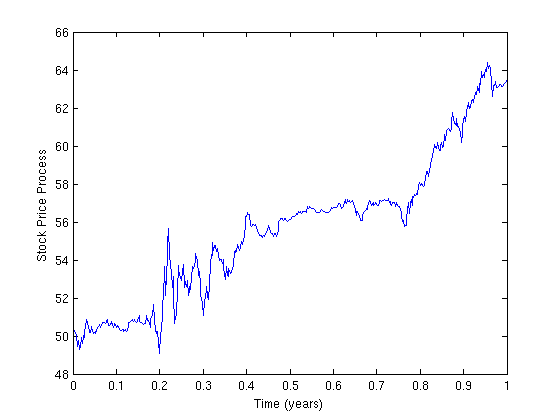
\includegraphics{Figures/sample_path.png}
 \caption{A sample path of the stock price. Initial values: $S_0 = 50$, $\sigma_0 = 0.2$, $\xi_0 = 0.2$. Parameter values: $\mu = 0.1$, $p = 3$ and $\alpha = 2$.}
\end{figure}

To study the influence of the parameters $p$ and $\alpha$ on the stock price process, the simulations are carried out such that one of the parameters is fixed while the other one is let to vary.
The results for the $p$ parameter are shown in Figure 2.
\clearpage

%FIGURE 2
 \begin{figure}[h]
 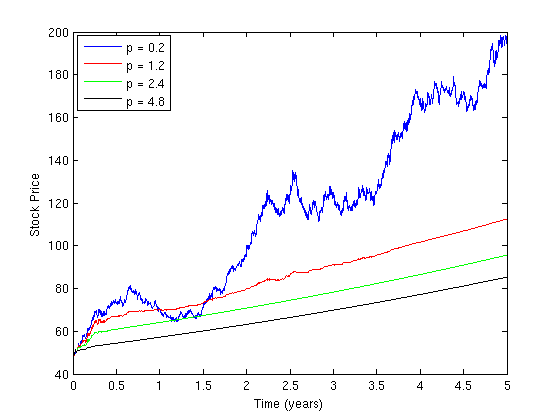
\includegraphics{Figures/p_effect.png}
 \caption{The influence of the parameter $p$ in the stock price.}
\end{figure}
In the case of parameter $\alpha$, we first study the influence it has on the behavior of the instantaneous and average volatility, Figure 3 and 4 respectively.

%FIGURE 3
 \begin{figure}[h]
 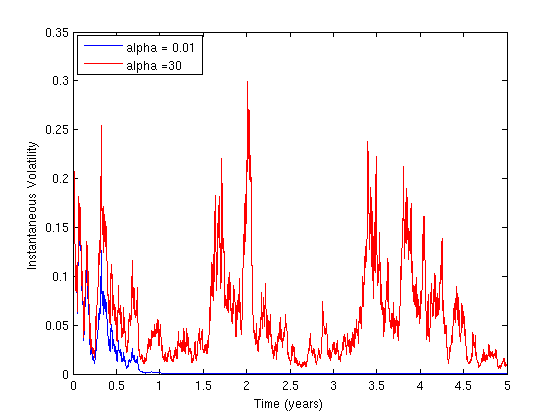
\includegraphics{Figures/alpha_effect_sigma.png}
 \caption{The influence of the parameter $\alpha$ in the instantaneous volatility.}
\end{figure}

%FIGURE 4
 \begin{figure}[h]
 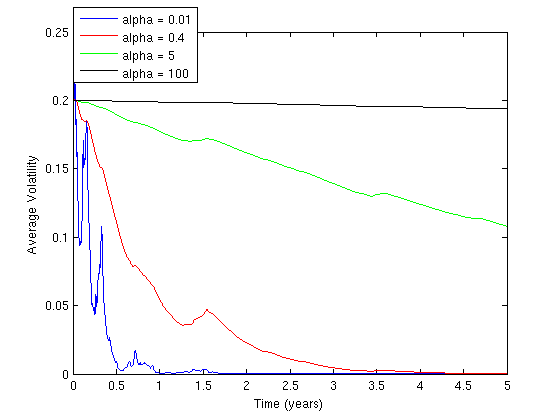
\includegraphics{Figures/alpha_effect_xi.png}
 \caption{The influence of the parameter $\alpha$ in the average volatility.}
\end{figure}

%FIGURE 5
 \begin{figure}[h]
 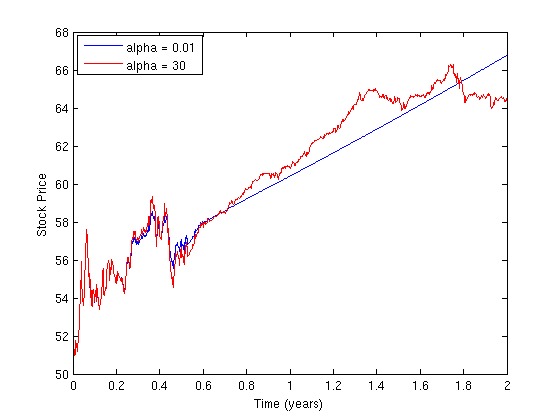
\includegraphics{Figures/alpha_effect_S.png}
 \caption{The influence of the parameter $\alpha$ in the stock price.}
\end{figure}
\clearpage
%MILSTEIN SCHEME
\subsection{The Milstein Scheme}
In general, if the stochastic process $X_t$ is given by the model:
\begin{equation}
dX_t = a(X_t,t)X_t dt + b(X_t,t) X_t dW_t
\end{equation}
then its Euler scheme reads:
\begin{equation}
X_{n+1} = X_n + a X_n \Delta n+ b X_n \, \Delta W_n\\ 
\end{equation}
\paragraph{}
The Milstein method is obtained by adding another term to (9), namely: 
\begin{equation}
\frac{1}{2} \, b \, b' \,((\Delta W_n)^2 - \Delta n)
\end{equation}

In the case of system (1), the Milstein scheme gives:

\begin{eqnarray}
\nonumber
S_{n+1} = S_n +\mu S_n \Delta n+ \sigma_n S_n \, \Delta W_n^1 + 0.5 \, \sigma_n^2 \, S_n \, ( (\Delta W_n^1)^2 - \Delta n) \\
\sigma_{n+1} = \sigma_n - (\sigma_n - \xi_n) \Delta n + p \sigma_n \, \Delta W_n^2 + 0.5 \, p^2 \, \sigma_n \, ( (\Delta W_n^2)^2 - \Delta n)\\
\nonumber
\xi_{n+1} = \xi_n + \frac{1}{\alpha} (\sigma_n - \xi_n) \Delta n
\end{eqnarray}

\subsection{Order of Convergence}
It has been shown that Euler method has the order of strong convergence equal to $0.5$, while Milstein method converges with the strong order of $1$.\\
Here we show that this is indeed the case, by simulating many paths of the stock process.\\ Since the analytic solution does not exist, it is approximated with Milstein scheme with a very small time step - at least 32 times smaller than the smallest time step used for approximation\footnote{Here the analytic solution is approximated with time step equal to $0.0001$. Then the following time steps are compared: $0.0032$, $0.0064$, $0.0128$ and $0.0256$.}.
The result is shown in Figure 6.
%FIGURE 6
 \begin{figure}[h]
 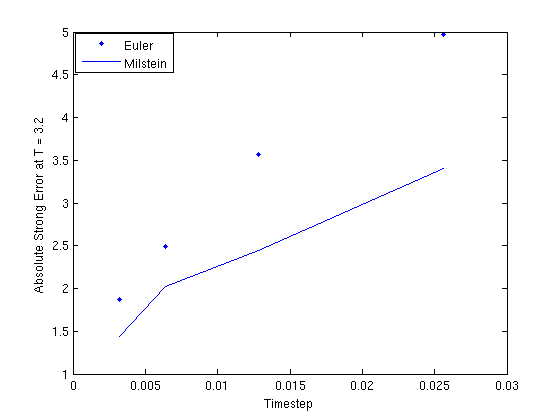
\includegraphics{Figures/euler_milstein.png}
 \caption{The strong convergence behavior of Euler and Milstein schemes.}
\end{figure}
\clearpage

In the weak sense, both methods have the same order of convergence equal to $1$.  This is shown in Figure 7 (Euler) and Figure 8 (Milstein).
%FIGURE 7
 \begin{figure}[h]
 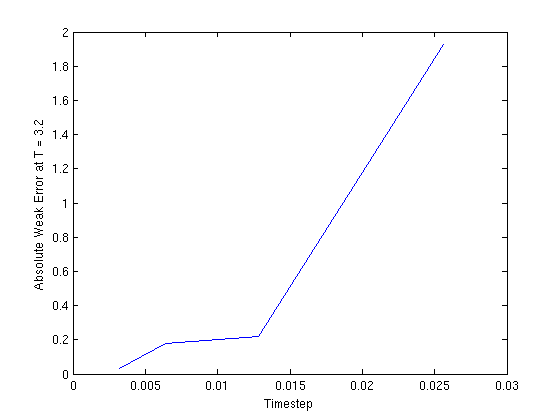
\includegraphics{Figures/euler_weak.png}
 \caption{The weak convergence behavior of the Euler scheme.}
\end{figure}
\clearpage

%FIGURE 8
 \begin{figure}[h]
 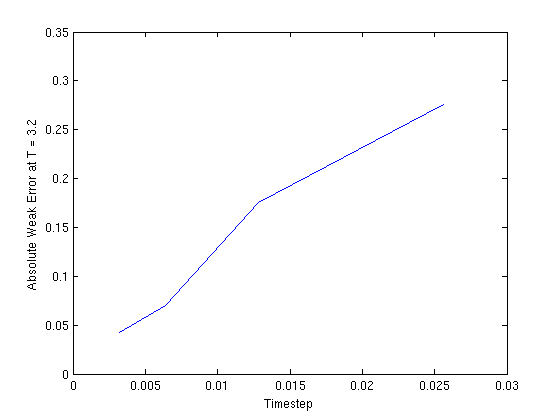
\includegraphics{Figures/milstein_weak.png}
 \caption{The weak convergence behavior of the Milstein scheme.}
\end{figure}
\clearpage

\section{Pricing a Put Option on a Stock that Follows Model (1)}

A European put option is the right to sell the share at time $T$>$0$ for a price $K$. It is assumed that Black Scholes formulas can be used to determine the price of a put option. 
We consider a level-click fund where \textbf{we buy put options at the money with T = 5 years to expiration, to protect our shares}\footnote{Here I am confused:\\
Suppose the share price is $S = 50$, the interest rate is $r = 0.05$, the volatility is $0.3$, expiration time is $T = 5$ years and strike is $K = 50$. \\Say I have $20$ shares and I am willing to buy $x$ number of at-the-money puts to protect my shares. \\I can use the Black Scholes to find the price of such a put, in this case it is: $p = 6.9$ \$.\\\\
My question is: How do I find the number $x$?\\\\
Suppose $x = x_0$ and the price of the put is $p = p_0$, then I would need $x_0 \times p_0$ dollars to create the portfolio. Then this amount of money should remain constant during the $5$ years.
}.
\\
If the shares have increased by $l = 10$\%, we sell the put options and a few shares and buy new put options at the money with T = 5 years to expiration. The total amount of money should remain constant.

\begin{itemize}
\item
Assume that the BS model is a realistic model for the stock price. Approximate by simulations the probability distribution of the value of the portfolio (shares + put options) after 5 years. Discuss the influence of the percentage $l$.
\item
Now assume that the model ($1$) is the correct model for the stock price. The options however are still available on the market for the Black Scholes prices. Approximate again by simulations the probability distribution of the value of the portfolio after 5 years. How can you gain money with this knowledge?
\end{itemize}
%\bibliographystyle{plain}  % other styles: abbrv, alpha, astron ...
%\addcontentsline{toc}{section}{References}
%\bibliography{thesis}     % Here, bibfile.bib is the bibliography file
                           % for your thesis.
                           % You need to LaTeX your thesis, then
                           % bibtex bibfile (NO .bib extension in the
                           % command)
\end{document}  